\chapter{Implementation}
\label{ch:implementation}

This chapter will serve as the overview of the final implementation of this algorithm.
As it was previously said, this algorithm is a part of the verification tool \text{VeriRego}, developed by the research group \text{VeriFit}.

As the source code of the targetted Open Policy Agent (OPA)\footnote{
    The Open Policy Agent is publicly available at \url{https://github.com/open-policy-agent/opa}.
}
is written in the programming language \textsc{Go}, a lot of the infrastructure is already prepared when choosing this language as the base for \text{VeriRego}.
Most importantly, this publicly available source code contains modules for translating the policy specification in Rego into a Syntax Tree (ast) and compiling of such ast into more sophisticated form (see module \text{compile}).

In this chapter, we will peak behind the curtain of the most important steps of the desired transformation.
That is, the type inference, generating of the SMT-LIB compliant sort, expression transformation, and the general structure of the implemented work.

\section{Type Inference}
A big role in the whole process of transforming Rego policies into SMT-LIB format is the type inference.
The most relevant reason is that the Rego Policy Language is dynamically typed, which means that each variable does not have its type specified.
The consistency of variables is not enforced at all by the system, if all the occurences in expressions hold true for the distinct variables.
Even with this treterous possibility, most of the times, the actual variable type is not that complicated, which means that for most of the part, it is transformable, as long as it is known.

For each variable the type inference looks at all its occurences, which are either assignments into it, which strongly imply its type, or expression usages, which weakly imply its type.
When multiple distinct types are implied for the given variable, it is noted as having the \text{Union} type.


\section{SMT-LIB generated types}

The most important fact to note is that object and array variables can store other variables inside them.
This implies that the generated type needs to be somehow recursive, which unfortunately deems the generated SMT code unresolvable even with the simplest of examples.
To counteract this, we employ the knowledge from the Type Inference, to cut off the maximal type depth.
With this specification, the atomic data types \text{String}, \text{Integer}, \text{Boolean}, and \text{Null} have a depth of $0$.
The depth of a structured datatype (object or array) is then equal to the maximal depth of its elements $+ 1$.

\begin{figure}
    \centering
    \label{fig:smt-types}
    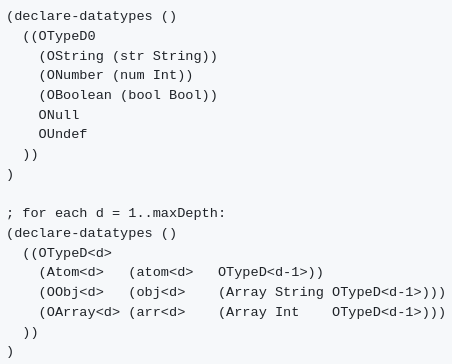
\includegraphics[width=0.7\textwidth]{figures/smt-generated-types.png}
    \caption{Generated datatypes for the SMT interpretation.}
\end{figure}

Every time a Rego policy and the input document are parsed, the type inference finds the maximum depth $d_{max}$.
The datatypes created are shown in the Figure \ref{fig:smt-types}.


\section{JSON Schema}
As mentioned in the previous Chapter, the final program is going to be able to operate on symbolic input documents.
For this purpose, it is recommended to use the \text{JSON Schema} format, which allows to specify certain keys mapping only to a specific type, or their union.

\paragraph{Types.}
Types are specified with setting the key \text{"type"} to one of the following JSON Schema types:
\begin{itemize}
    \item \text{"object"}
    \item \text{"array"}
    \item \text{"string"}
    \item \text{"integer"} or \text{"number"}
    \item \text{"boolean"}
    \item \text{"null"}
\end{itemize}
To declare a type as union, an array of types is used, e.g., \text{["string","null"]}.

% \paragraph{Combining Schemas.}

